%#########################################
% For 140601 GitHub Kaigi
% title: GitHubで行うreproducible research
%#########################################
\documentclass[dvipdfmx, 14pt]{beamer}
\usepackage{pxjahyper, otf, mediabb, tikz, wrapfig}
\usepackage{pifont}
\usetheme{default}
\renewcommand{\kanjifamilydefault}{\gtdefault}
\renewcommand{\familydefault}{\sfdefault} % 欧文書体をHelveticaに
\setbeamertemplate{navigation symbols}{}
\setbeamertemplate{background canvas}{
\includegraphics[height=\paperheight]{bg}}
\setbeamerfont{title}{size=\huge, series=\bf}
\setbeamercolor{title}{fg=black}
\setbeamercolor{frametitle}{fg=black}
\setbeamerfont{alerted text}{series=\bf}
\setbeamercolor{alerted text}{fg=custom.fc}
\definecolor{custom.fc}{HTML}{F4F6F7}
\graphicspath{{../../src/}}
%#######*****####### titile #######*****#######***
\title{GitHubで行う\\reproducible research}
\author[瓜生]{\href{http://urush.postach.io}{瓜生真也}}
\institute[横国大院・環情]{横浜国立大学大学院 環境情報学府}
\subject{LT slide for GitHubKaigi@Shibuya}
\date{\scriptsize GitHub Kaigi(@Shibuya), June 1, 2014\\
\vspace{1em}
\href{http://github.com/uribo/rep-res-guideline}{github.com/uribo}
}
%#######*****#######*****#######*****#######***
\begin{document}

\frame{\titlepage}

{\usebackgroundtemplate{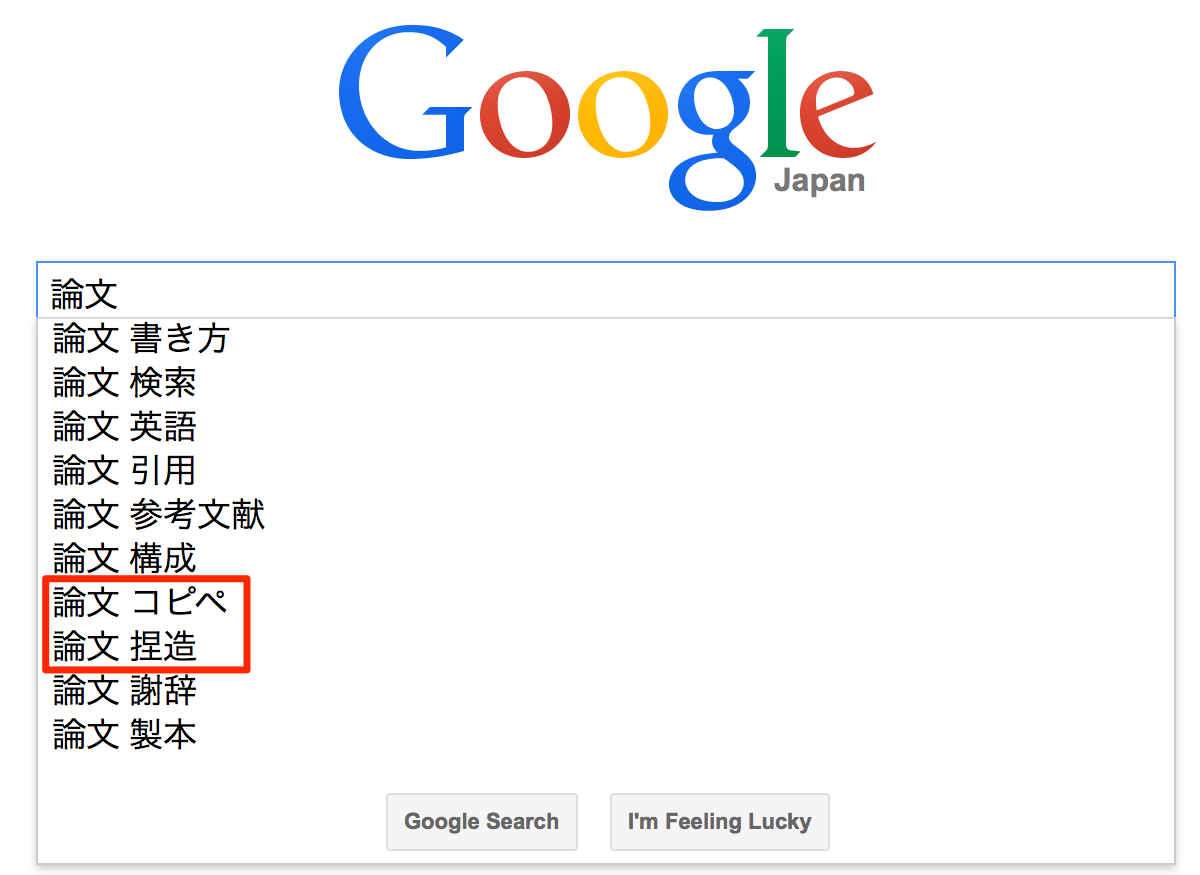
\includegraphics[width=\paperwidth]{gg-suggest}}%
\frame{}}%なぜ論文に再現性が必要なのか

{\usebackgroundtemplate{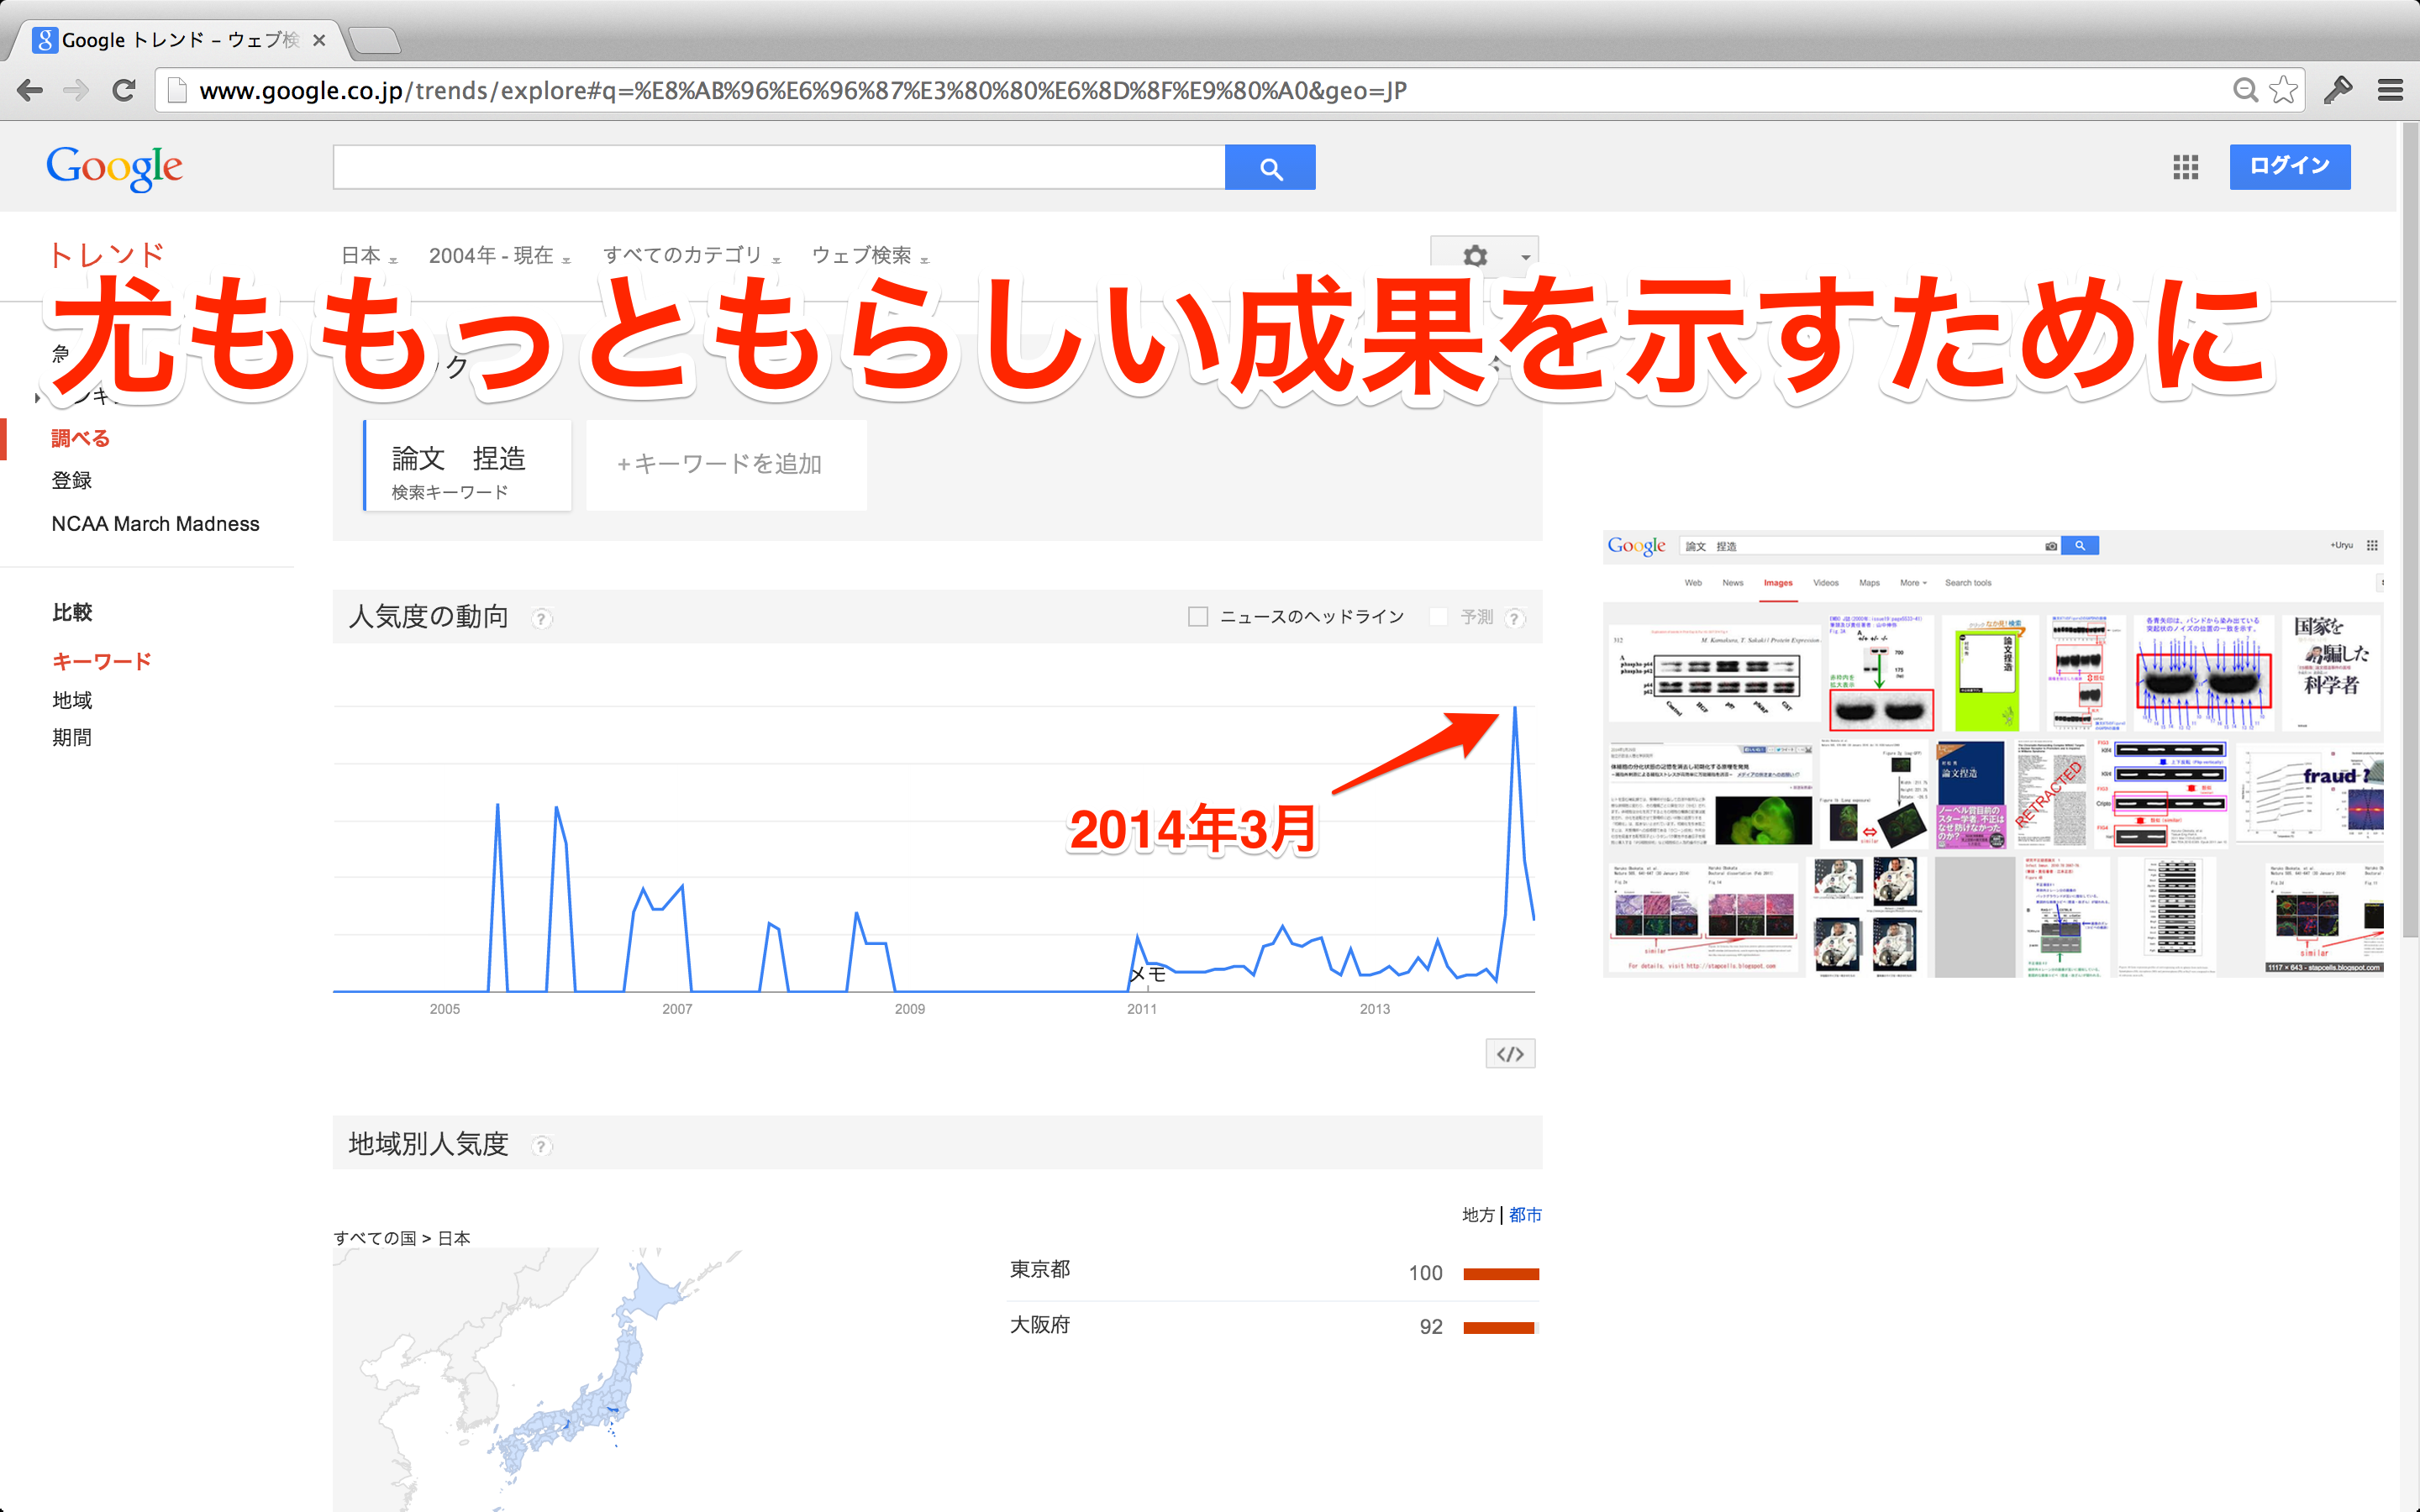
\includegraphics[width=\paperwidth]{gg-trends}}%
\frame{}}%尤ももっともらしい成果を示すために

\frame{
\frametitle{Reproducible Research (RR)}
  {\Large 再現可能な研究}\\
  \vspace{0.5em}
  論文に書かれている方法、条件で行えば、\\同様の結果が得られる
  \begin{wrapfigure}{o}[60pt]{60mm}
    
\includegraphics[height=3.5cm]{RR-icon}
  \end{wrapfigure}
  \vspace{0.5em}
  \begin{itemize}
  \setlength{\itemindent}{2em}
  {\Large
    \item[\ding{51}] \alert{客観性}
    \item[\ding{51}] \alert{明瞭性}
    \item[\ding{51}] \alert{妥当性}
  }\end{itemize}}
  
\frame{
  \frametitle{開発者と科学者で共通するもの}
  \begin{center}
  \vspace{-1.0em}
  {\tiny Prli{\'c}, A., and J. B. Procter. 2012. PLOS Computational Biology 8}
  
\includegraphics[width=8.0cm]{Prlic-and-Procter2012Plos}\\
  \end{center}
  \vspace{-1.0em}
  \begin{enumerate}
    {\small
    \item \alert{Don't Reinvent the Wheel}
    \item Code Well
    \item \alert{Be Your Own User}
    \item \alert{Be Transparent}
    \item \alert{Be Simple}
    \item Don't Be a Perfectionist
    \item Nurture and Grow Your Community
    \item Promote Your Project
    \item Find Sponsors
    \item Science Counts
  }\end{enumerate}
  }
%#######*****#######*****#######*****#######***
\frame{
  \frametitle{研究の流れ}
  統計解析と論文の執筆は鬼門
  \begin{center}
  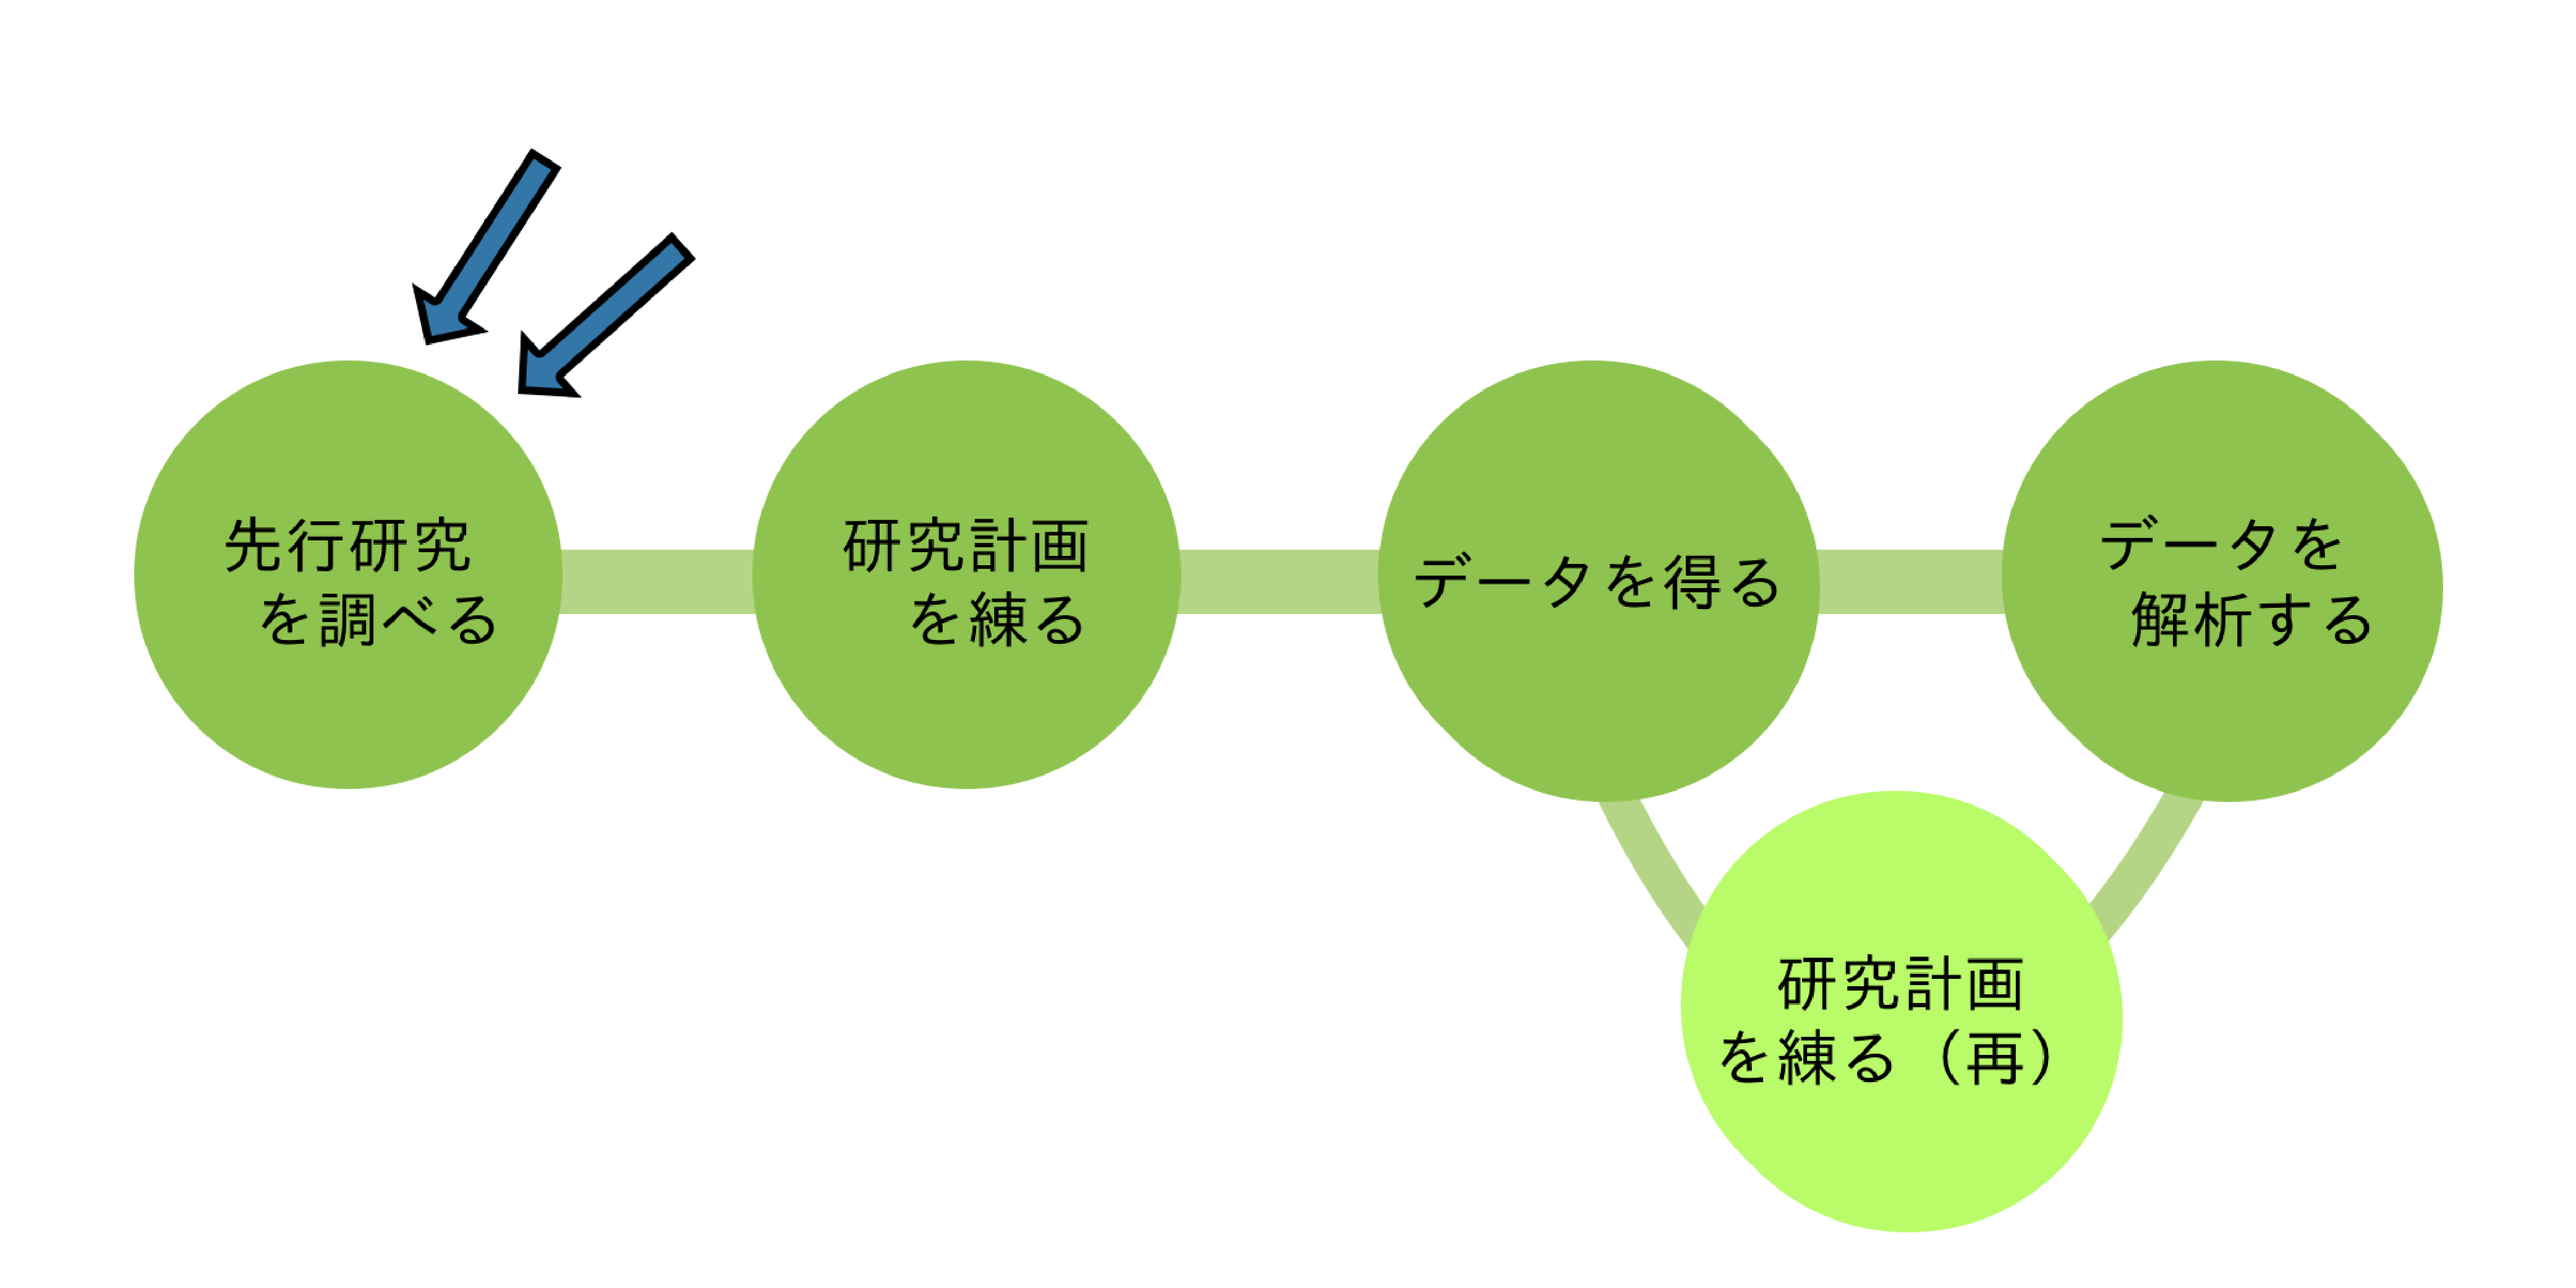
\includegraphics[width=11cm]{research-flow}
  \end{center}}

{\usebackgroundtemplate{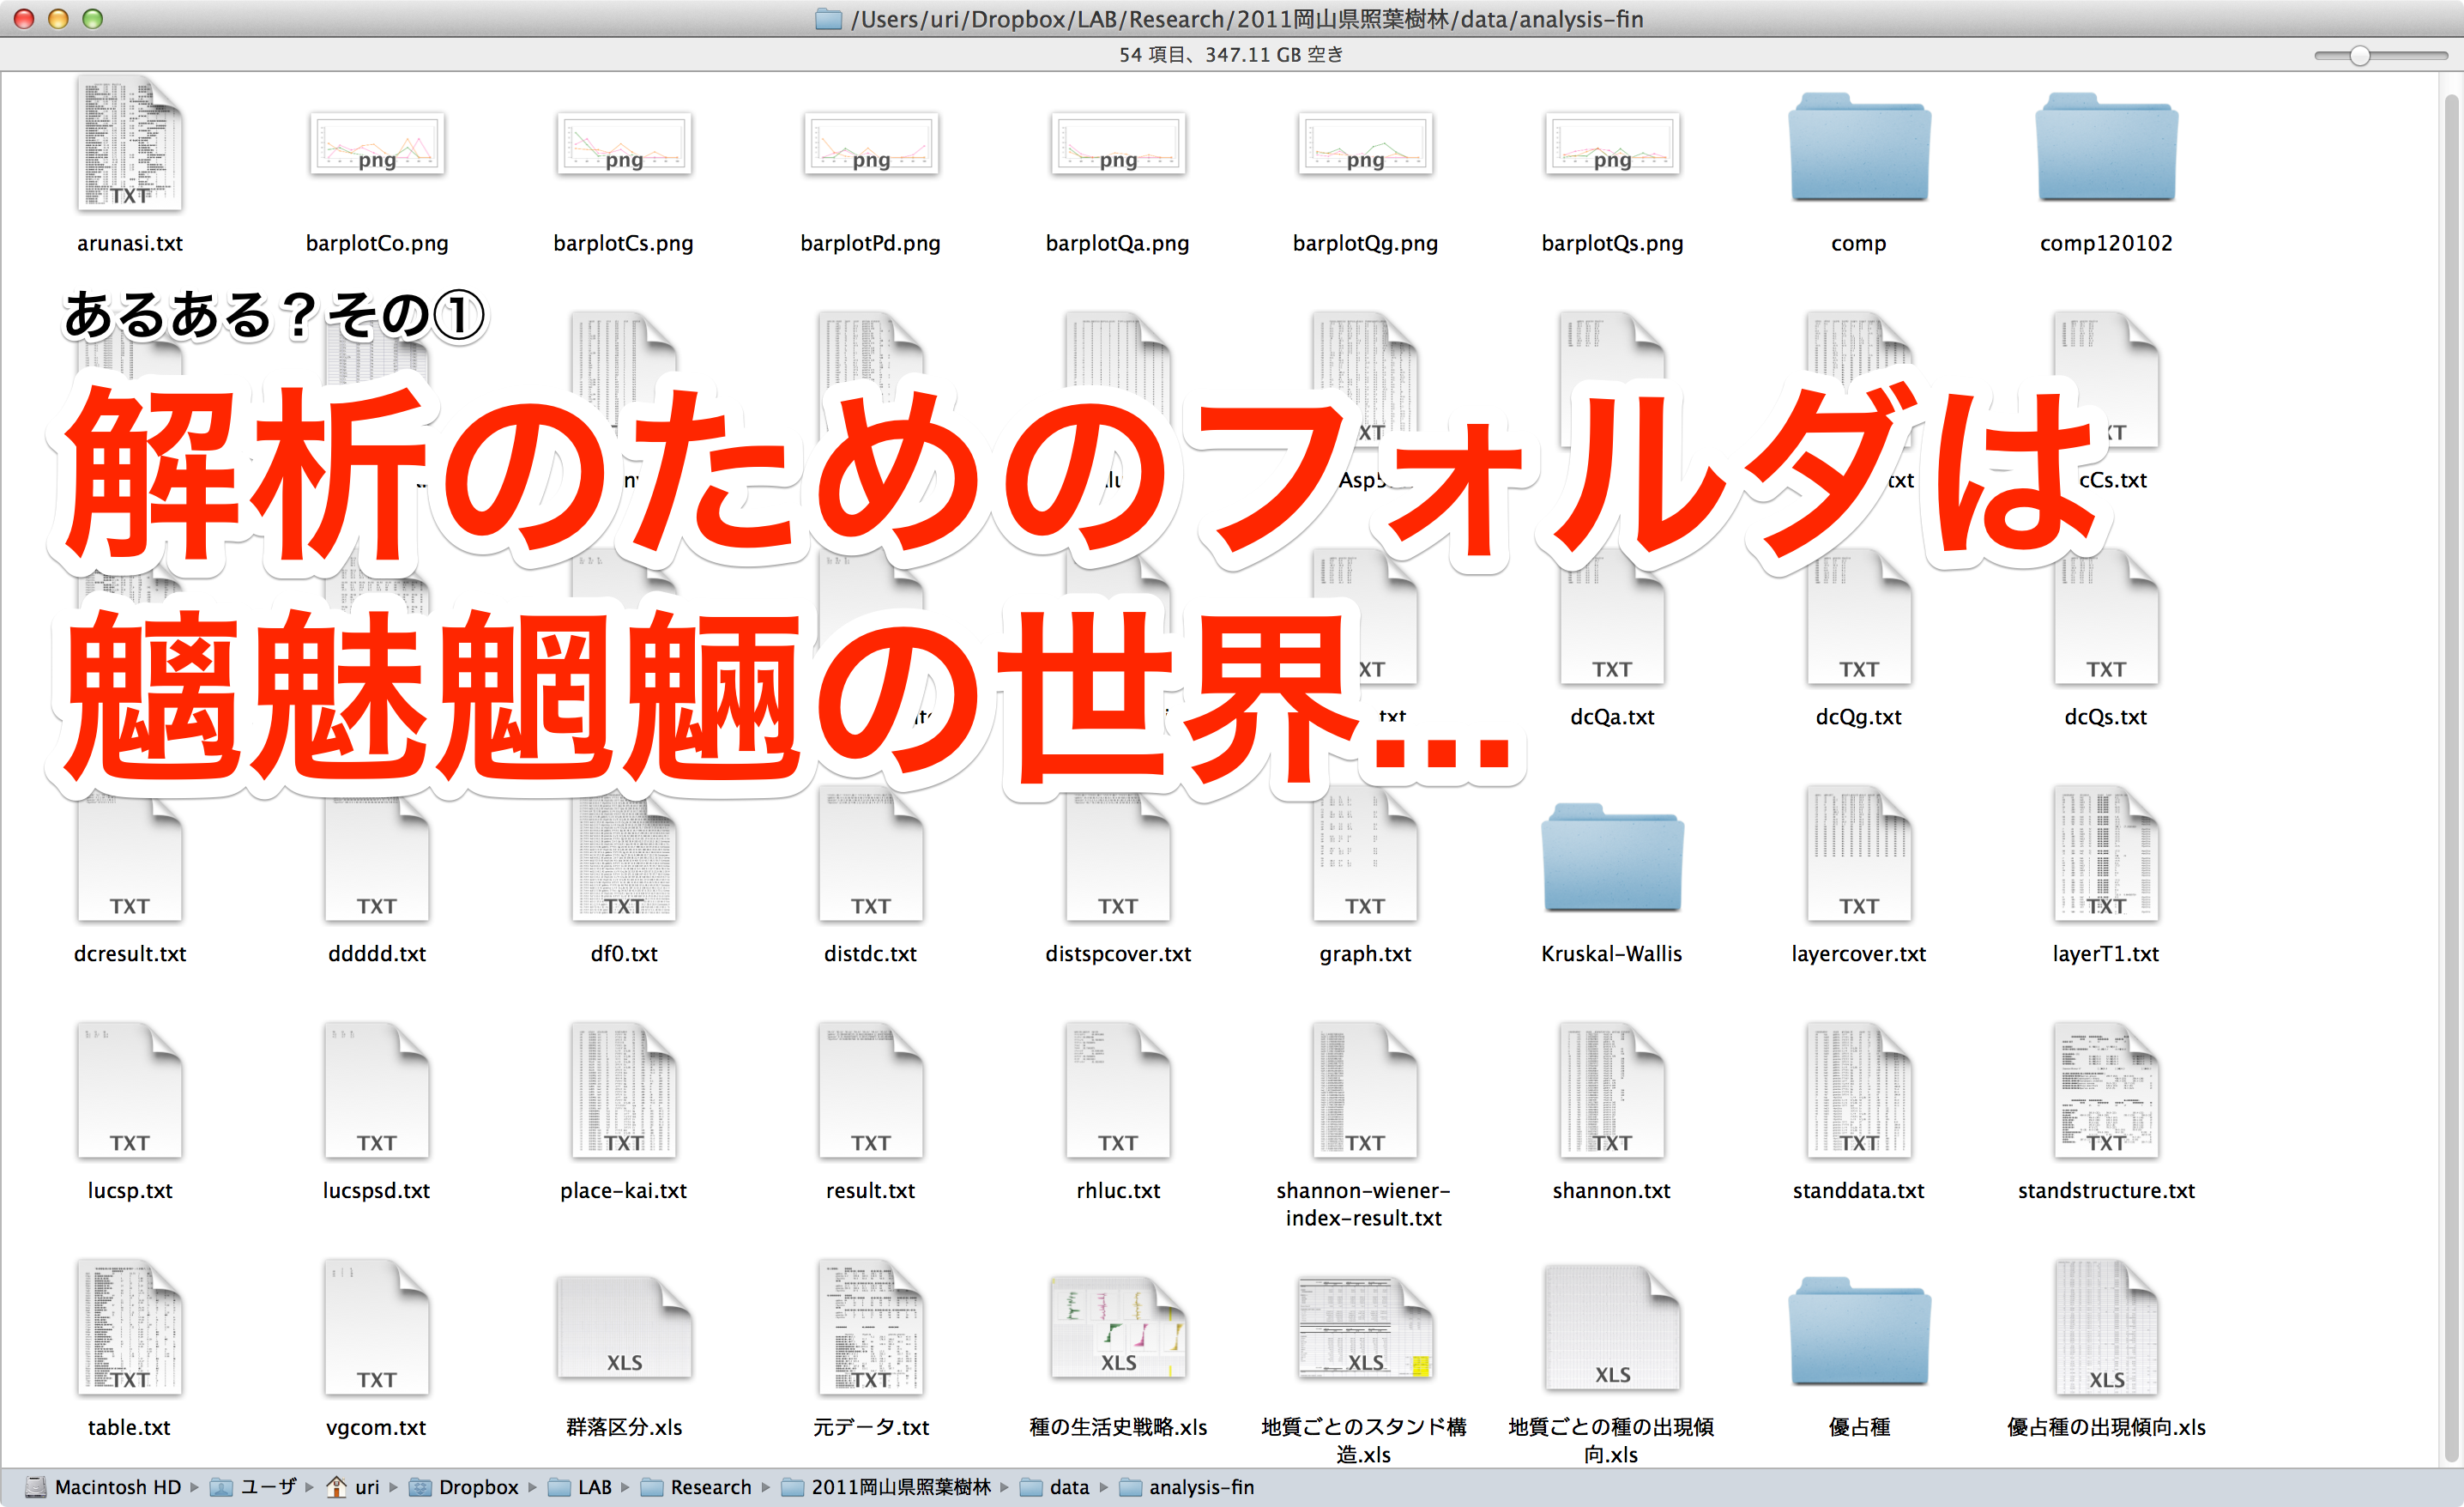
\includegraphics[width=\paperwidth]{misc-files}}%
\frame{}} %解析フォルダは魑魅魍魎の世界

{\usebackgroundtemplate{
\includegraphics[width=\paperwidth]{old-files-collection}}%
\frame{}} %過去のファイル

\frame{
  \frametitle{GitHubの特徴を活かしたRRな研究}
  ソーシャルコーディングの概念を研究に...
  \begin{center}
  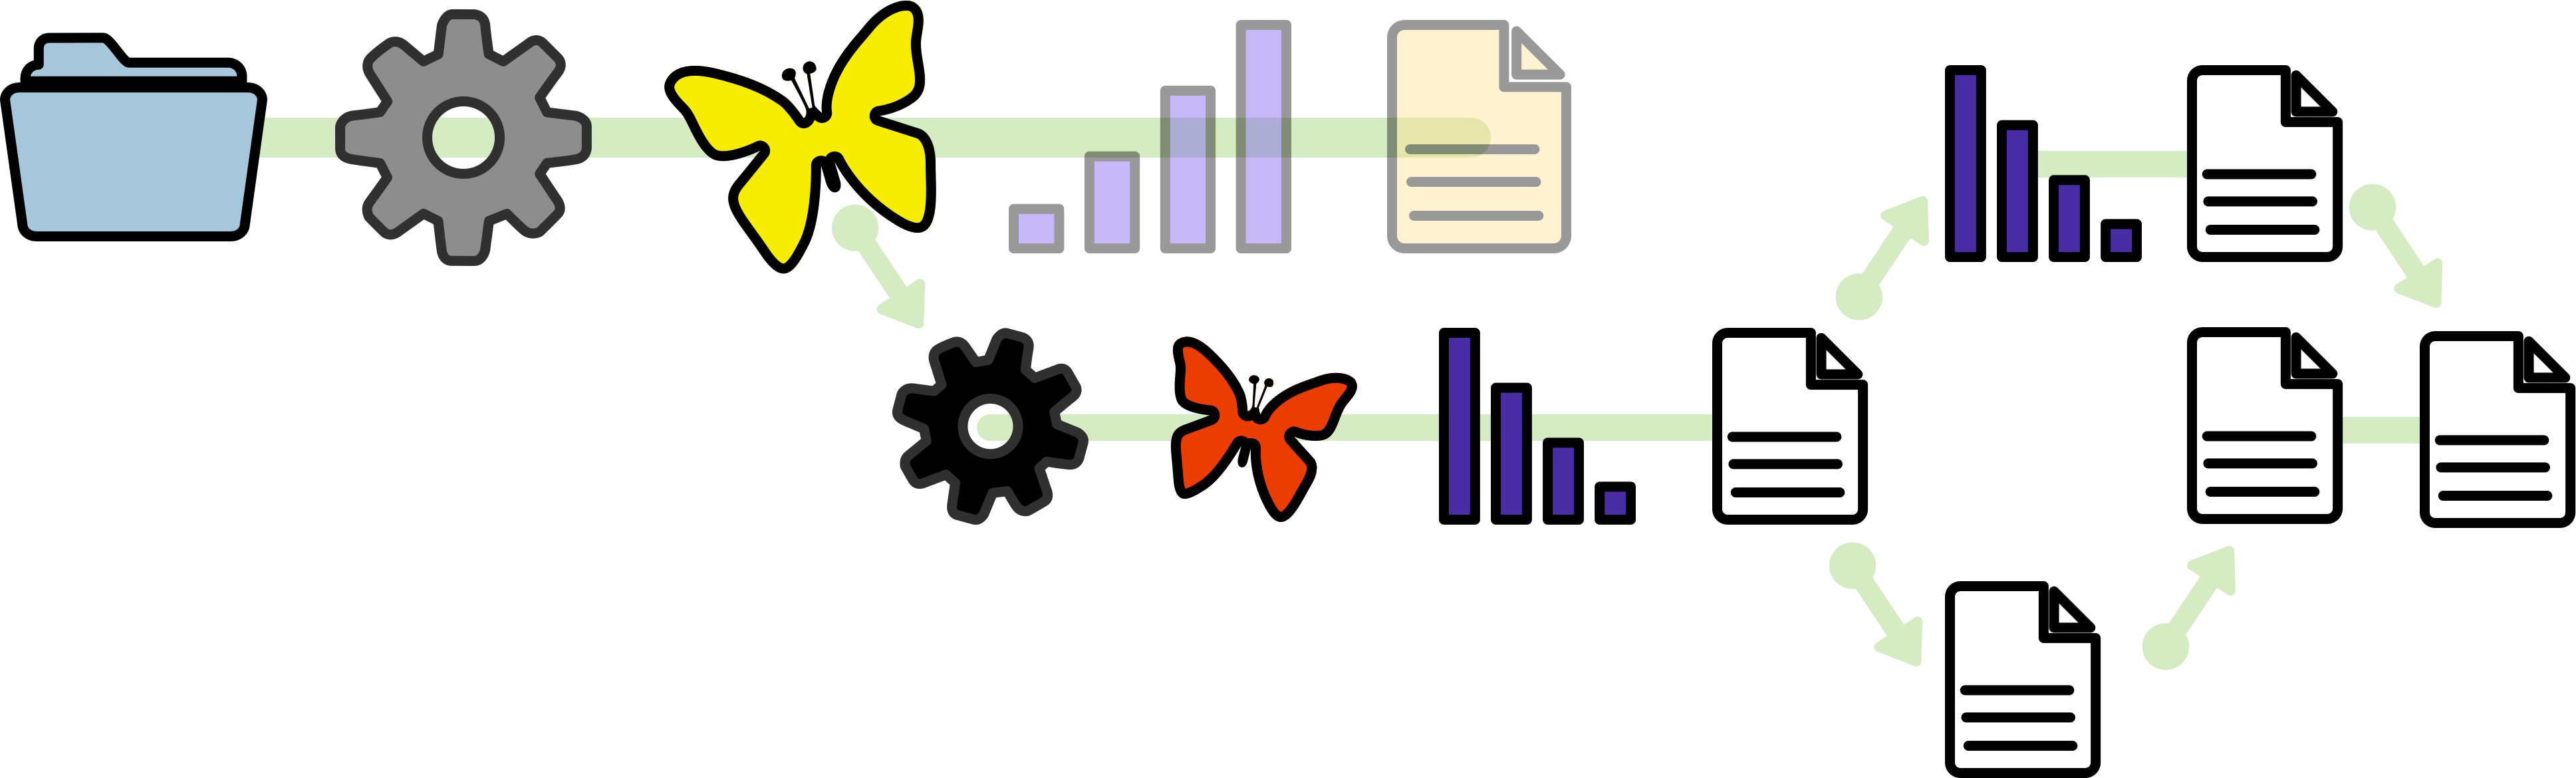
\includegraphics[height=3.0cm]{research-flow-branch}
  \end{center}
  \begin{itemize}
    \item テキストファイルをもとにした進行
    \item 進捗状況に応じたブランチの切り替え
    \item 用途を記述したコミットコメント
    \item バックアップ、差分確認は気にしない
  \end{itemize}  
}

\frame{
  \frametitle{データ解析: 
\includegraphics[height=0.7cm]{r-logo}}
  \vspace{0.5em}
  \begin{center}
  リポジトリ内のソースコード、データファイルを用いれば同様の結果が得ることができる\\
  \vspace{0.6em}
  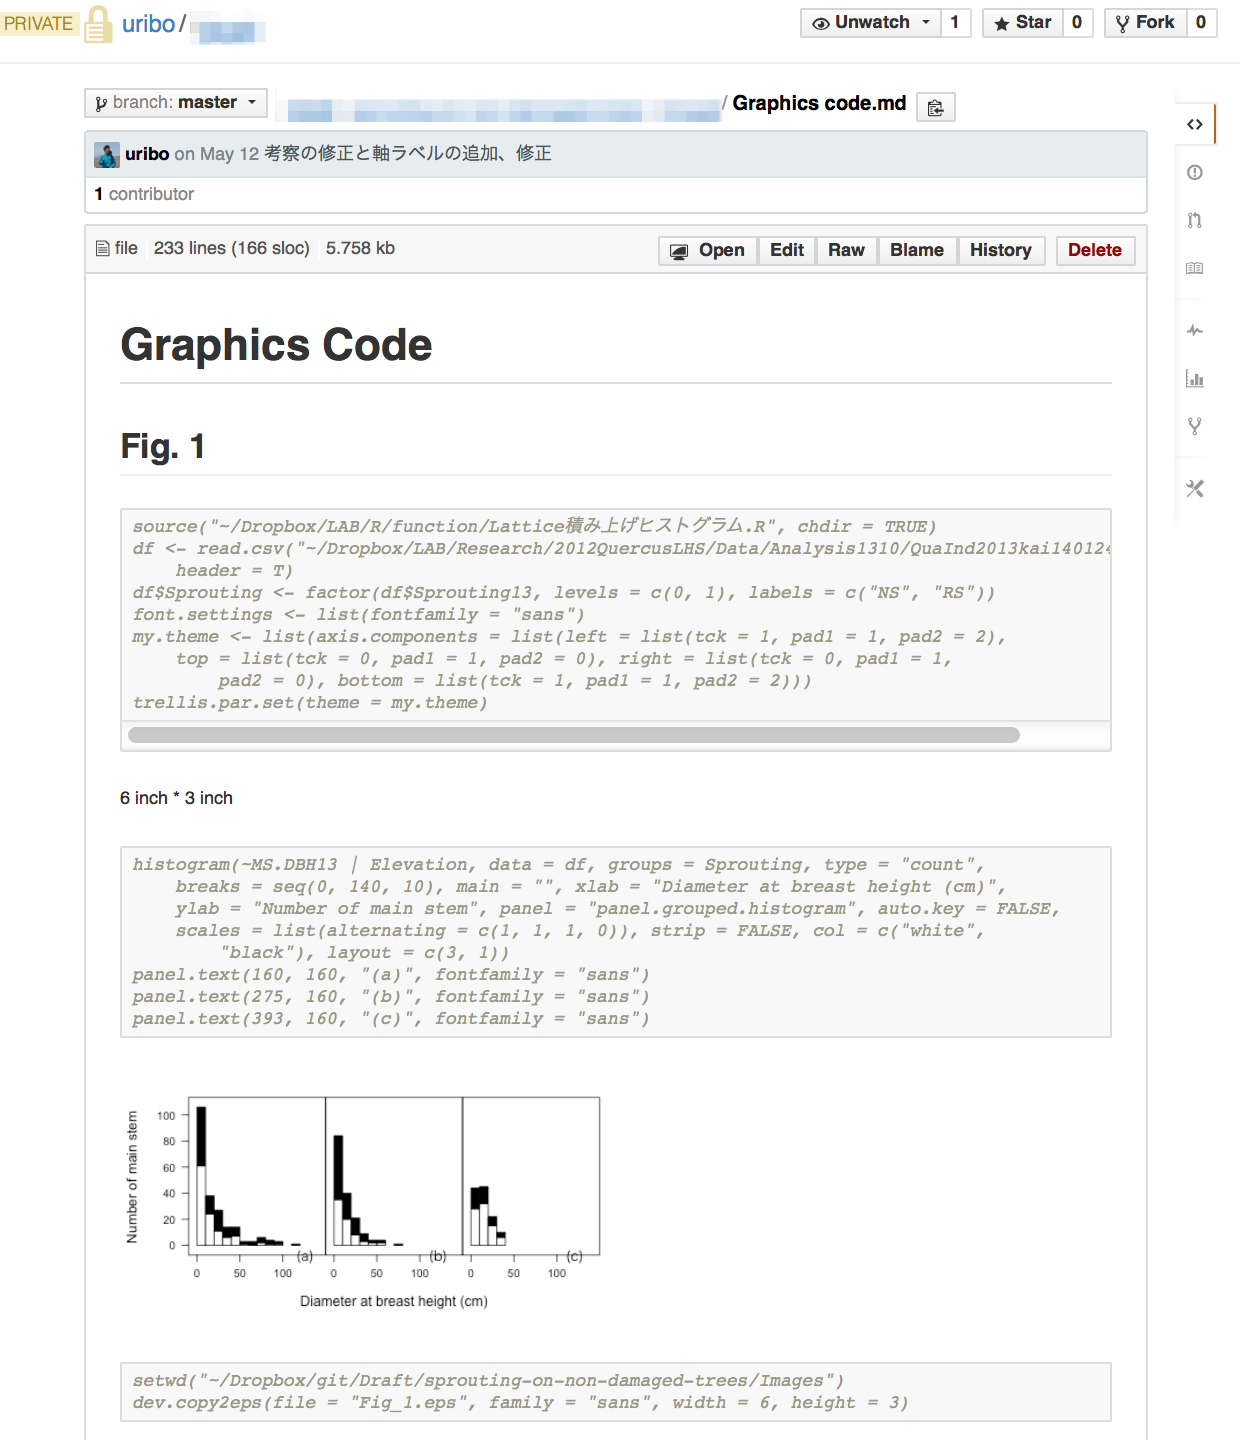
\includegraphics[height=6.0cm]{r-code-markdown}
    \end{center}}
    
\frame{
  \frametitle{論文執筆: 
\includegraphics[height=0.7cm]{latex-logo}}
  \begin{center}
  テキストファイルなので差分の確認が容易。\\必要があればバックアップから復元\\
  \vspace{0.6em}
    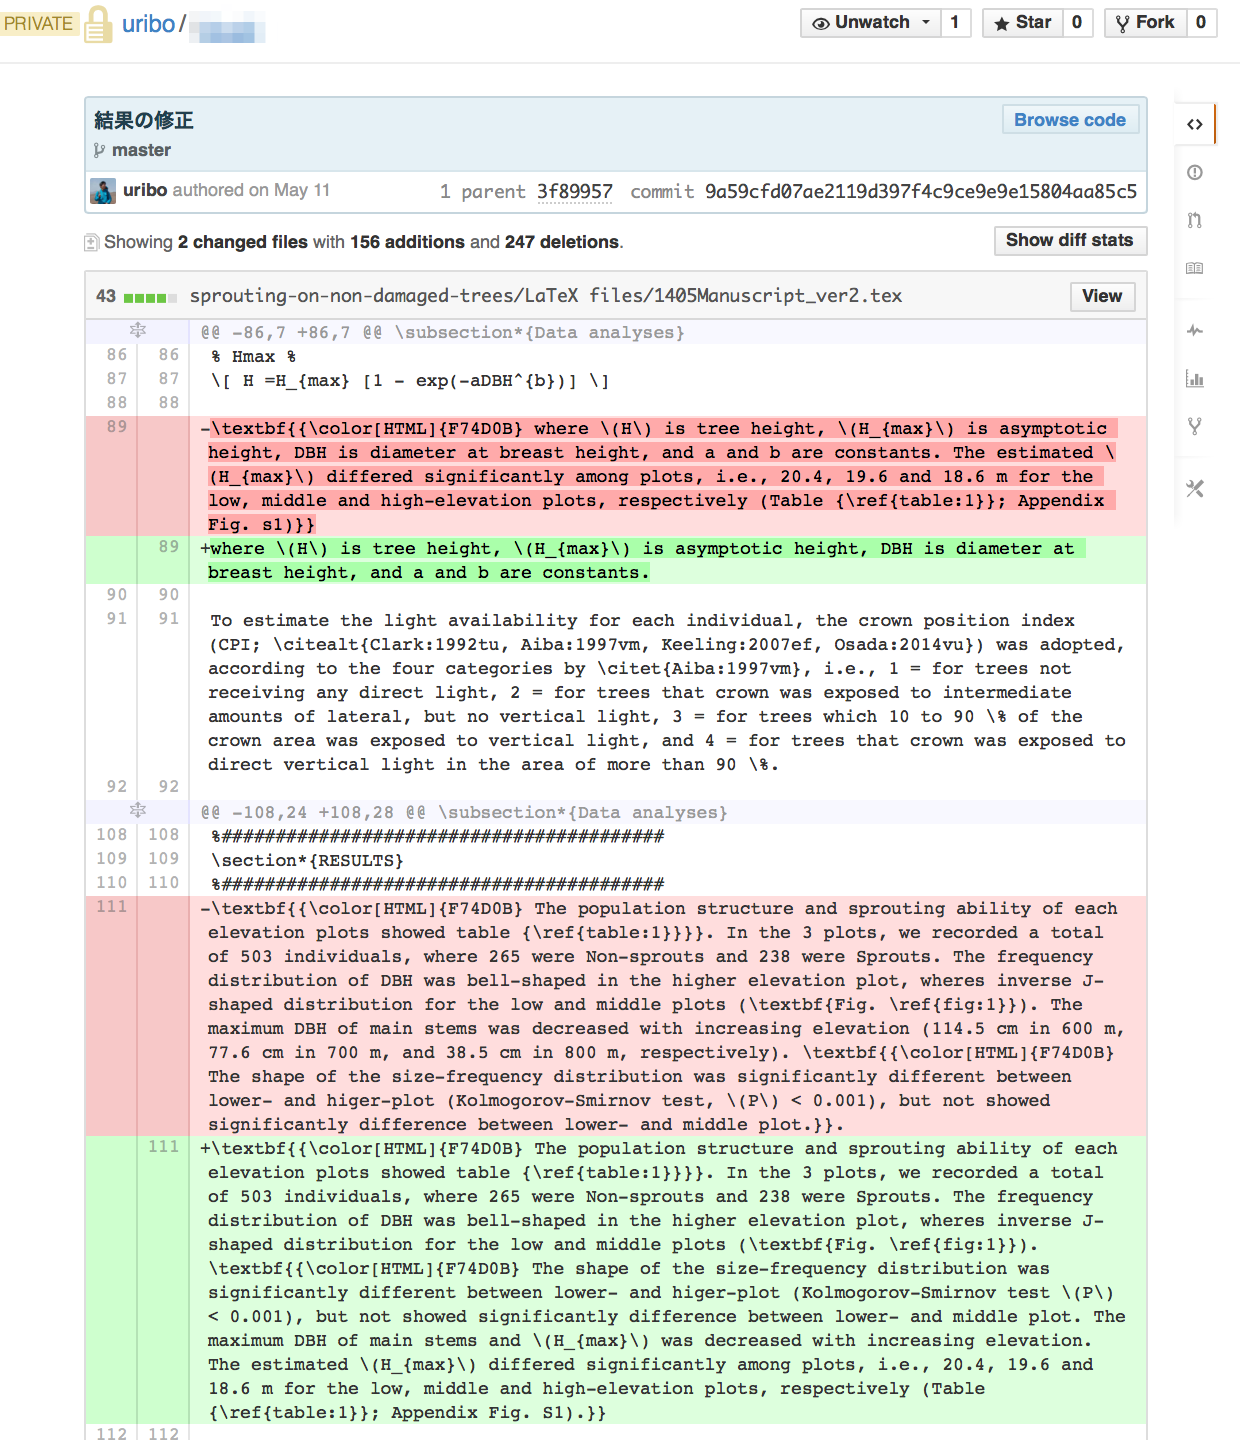
\includegraphics[height=6.0cm]{latex-revise}
  \end{center}}

\frame{
  \frametitle{Pull Request, Issuesを使った査読}
  \begin{center}
  
\includegraphics[height=5.0cm]{instruction}
  \end{center}}
%#######*****#######*****#######*****#######***
\frame{
  \frametitle{今後の展望と課題}
  \only<1>{
    \begin{itemize}
      \item Computational Scienceだけでなく、いかなる分野の研究にもreproducible researchの概念が必要
      \item Data analysisとWriting にGitHubが活用できる
      \item ソーシャルコーディングの概念は研究の再現性だけでなく、客観性や明瞭性を向上させる
    \end{itemize}}
  \only<2>{
    \begin{itemize}
      \item GitHubに生データを上げるのはどうなの? 安全?
      \item 査読は匿名、というのが原則... やめちまえ
      \item ソーシャルコーディングとの矛盾...
    \end{itemize}}}
\end{document}